%Licht allgemein
Licht lässt sich sowohl als Teilchen als auch als Welle auffassen.
Bei Prozessen, bei denen es auf das einzelne Lichtquant ankommt, ist eine Beschreibung als Welle nicht sinnvoll, so zum Beispiel bei dem Photoeffekt oder bei dem Comptoneffekt.
Prozesse, bei denen über große Anzahlen von Lichtquanten gemittelt werden kann, lassen sich durch eine Wellendarstellung beschreiben.
%Interferenz
\\Lichtwellen können dem Prinzip der Interferenz unterliegen.
Dabei überlagern sich mindestens zwei Lichtwellen.
Liegen zwei Wellenberge zweier Wellen mit gleicher Wellenlänge übereinander, addieren sie sich zu einem größeren Maximum.
Zwei Wellentäler addieren sich zu einem tieferen Wellental.
Diese beiden Phänomene fallen unter die konstruktive Interferenz.
Ein Wellenberg, der auf einem Wellental liegt, löschen sich Wellenberg und Wellental aus.
Dies wird destruktive Interferenz genannt.
Sind die Wellenlängen der beiden interferierenden Wellen nicht gleich, kommt es zu sogenannten Schwebungen und Wellenpakteten.
In diesem Versuch wird nur die Interferenz zweier gleicher Wellen betrachtet.
%Huygens
\\Das Huygens'sche Prinzip .
Es sagt aus, dass jeder Oszillator einer Welle der Ausgangspunkt einer neuen Elementarwelle sein kann.
Die einzelnen Elementarwellen summieren sich zu einer neuen Wellenfront.
Es kommt zur Interferenz der Elementarwellen.
Bei einer Grenzfläche, einem Einzelspalt oder einem Doppelspalt zeigt sich dieses Phänomen.
%Einzelspalt
\\Zunächst wird der Einzelspalt behandelt.
Dabei gibt es zwei Varianten die Beugung am Einzelspalt zu untersuchen; einerseits gibt es die Fresnel'sche Beugung, andererseits die Fraunhofer'sche Beugung (Abb. \ref{fig:fresnelfraunhofer}).
\begin{figure}[h!]
  \centering
  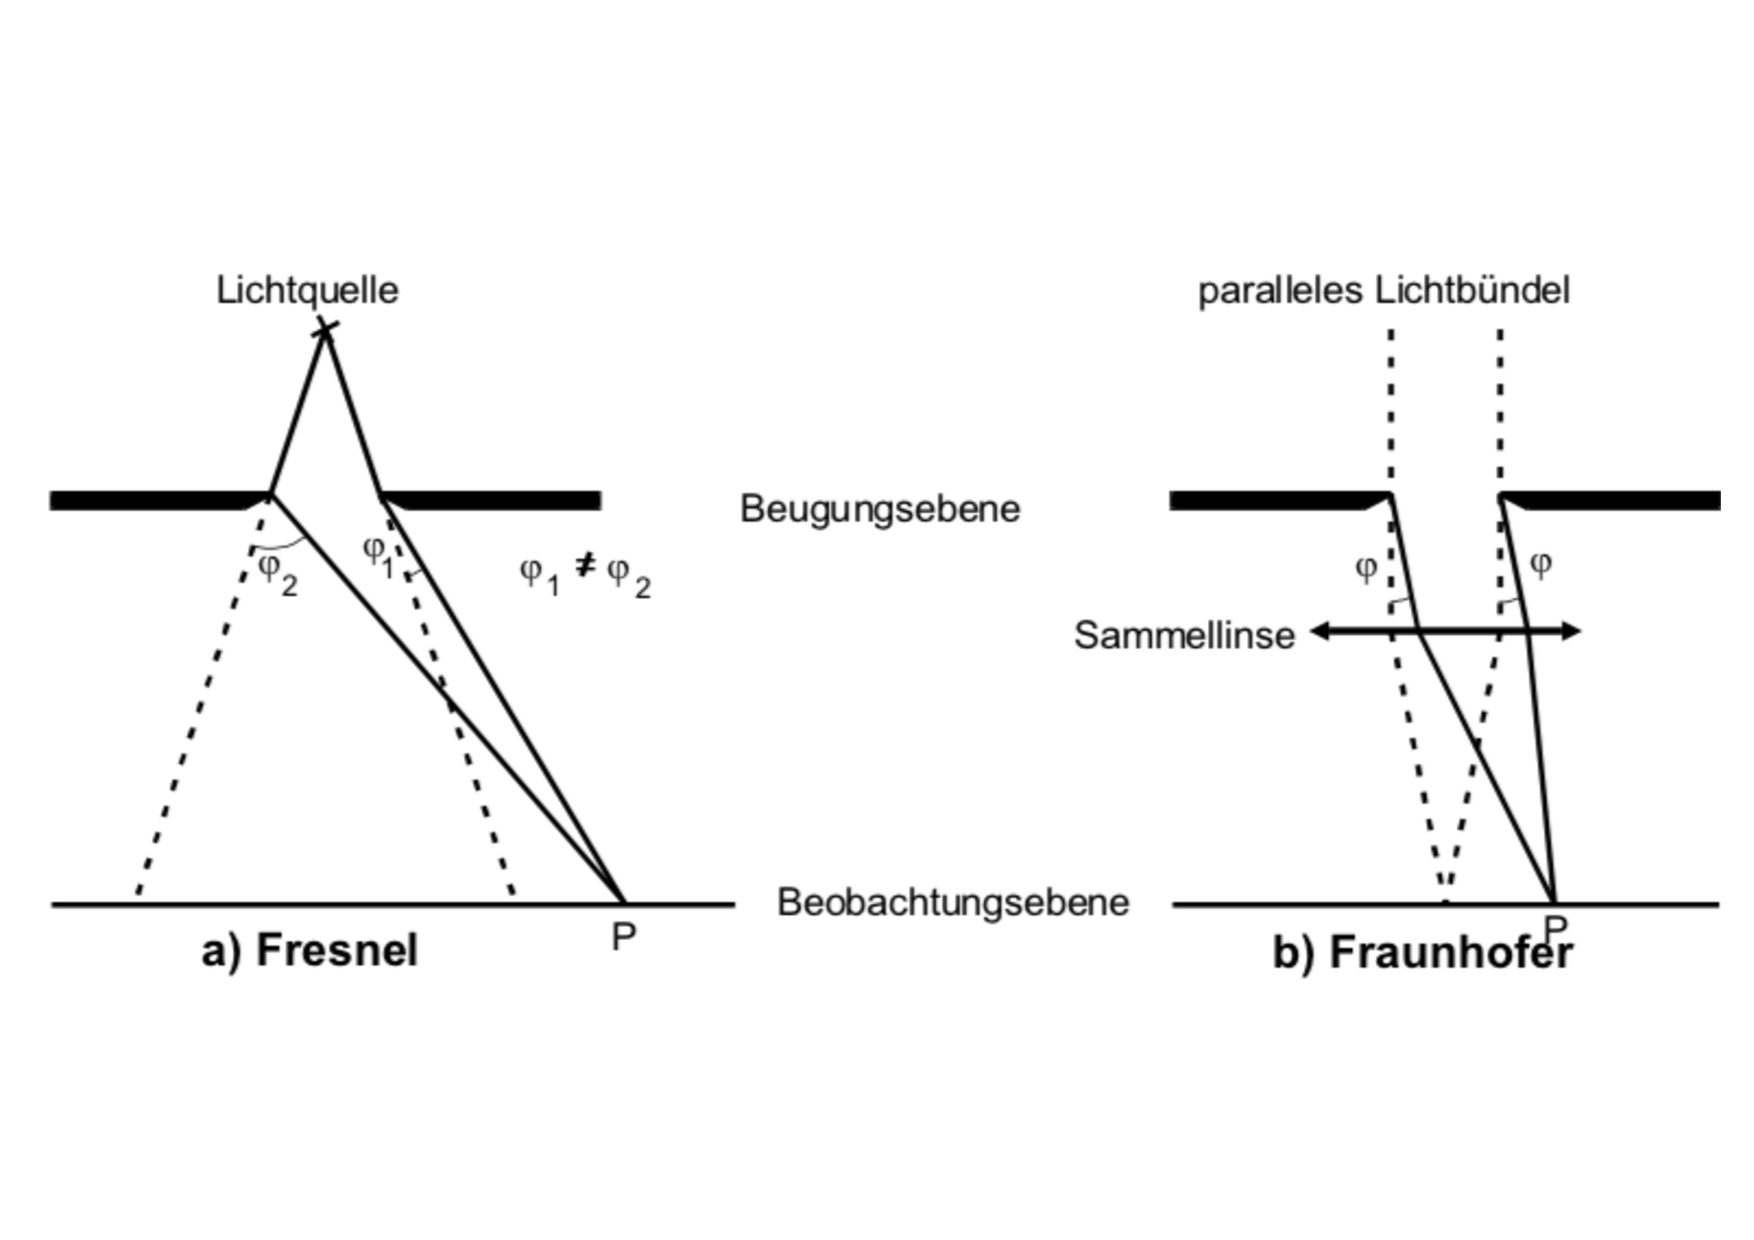
\includegraphics[width=\textwidth]{fresnelfraunhofer.pdf}
  \caption{Fresnel'sche und Fraunhofer'sche Beugung \cite{1}}
  \label{fig:fresnelfraunhofer}
\end{figure}
Bei der Fresnel'schen Beugung sind die Lichtquelle und die Bildebene nah an dem Spalt.
Die Fraunhofer'sche Beugung funktioniert mit größeren Abständen:
Die Lichtquelle ist so weit weg von dem Spalt, dass die einfallenden Lichtstrahlen parallel sind.
Auch die Bildebene ist weiter weg von dem Spalt.
In diesem Versuch wird die Fraunhofer'sche Beugung verwendet.
Der Strahlengang am Einzelspalt ist in Abbildung \ref{fig:einzelspalt} dargestellt.
\begin{figure}[h!]
  \centering
  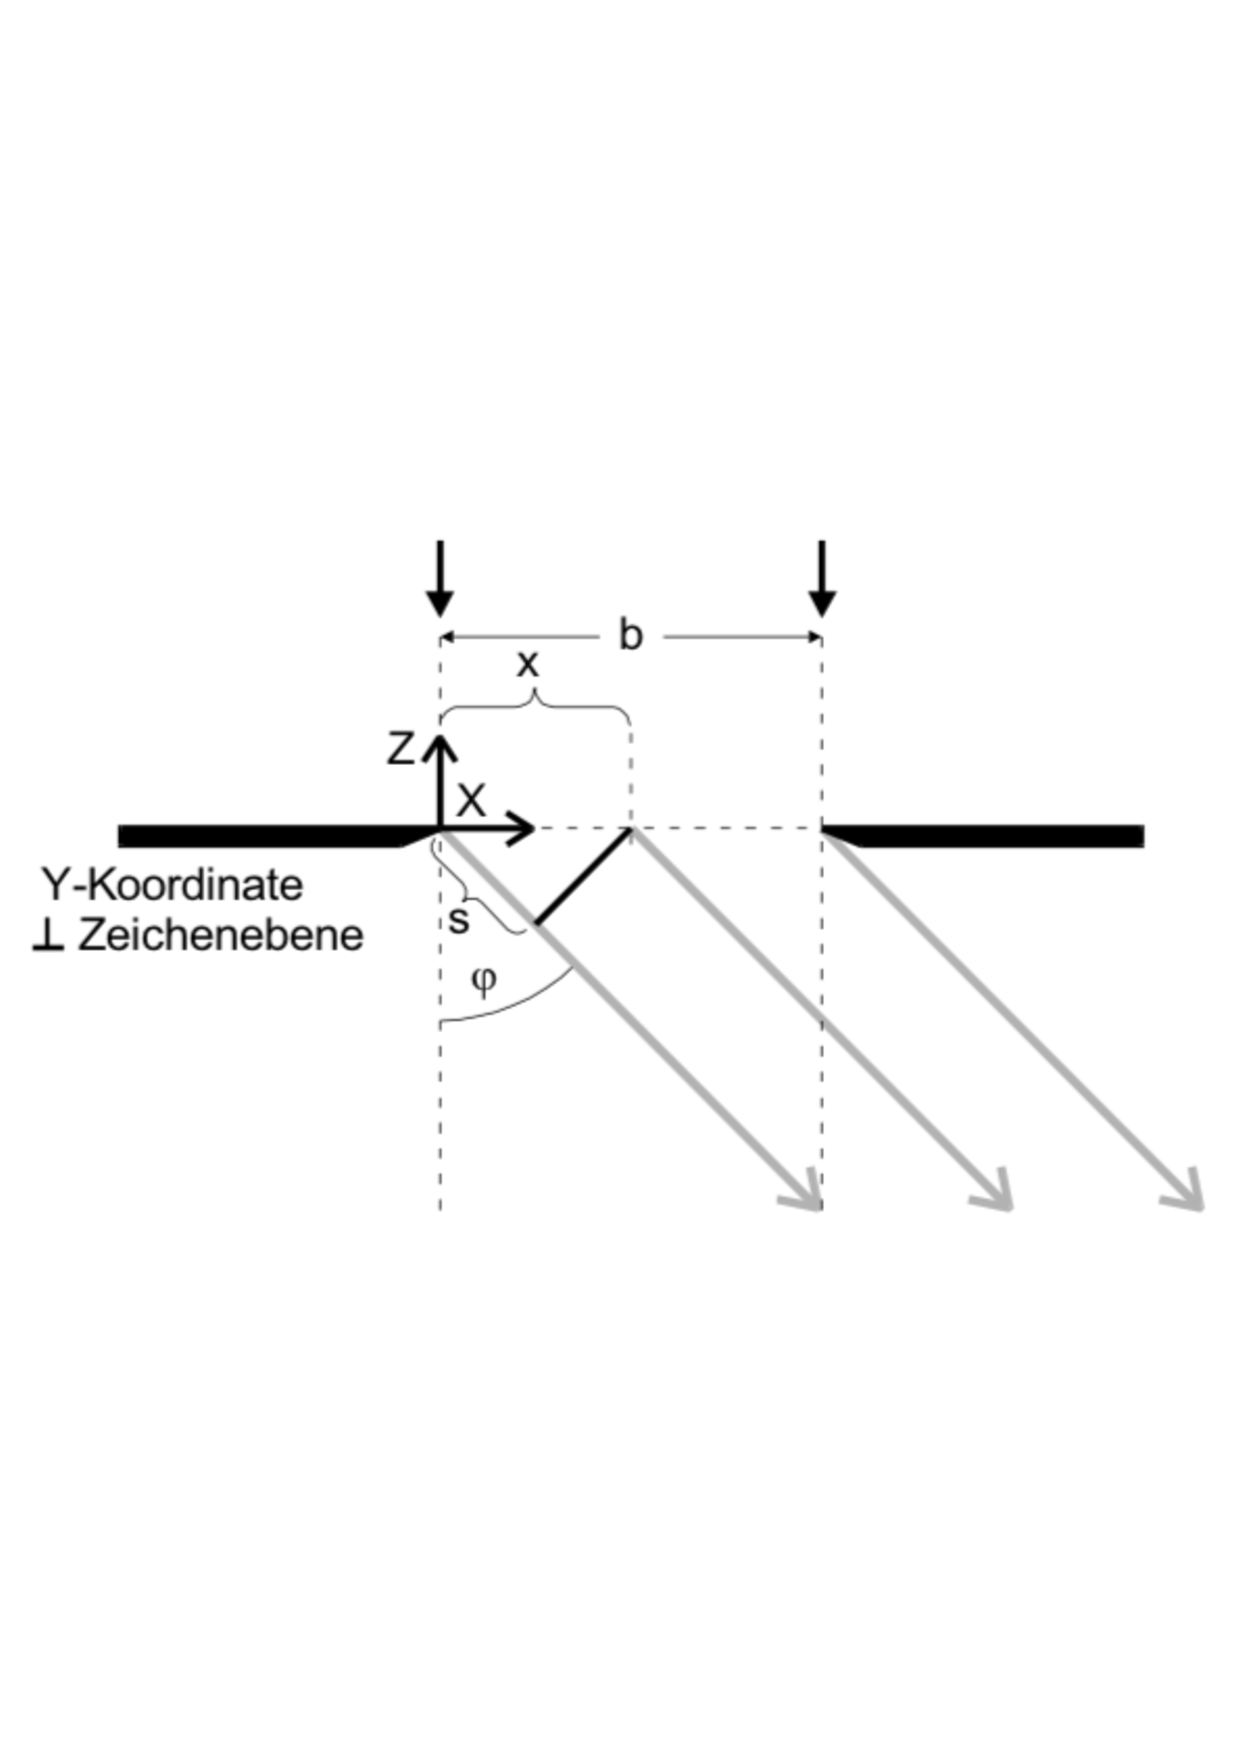
\includegraphics[width=\textwidth]{einzelspalt.pdf}
  \caption{Huygens'sches Prinzip am Einzelspalt \cite{1}}
  \label{fig:einzelspalt}
\end{figure}
Dabei ist zu erkennen, dass bei einer Beugung um den Winkel $\varphi$ ein Gangunterschied zwischen den Strahlen entsteht.
Eine Lichtwelle kann hier die Form
\begin{align*}
  A(z, t) = A_{0} \exp{ \left[i \left( \omega t - \frac{2 \pi z}{\lambda} \right) \right]}
\end{align*}
Die entstehende Phasendifferenz beim Gangunterschied $s$ zwischen zwei Strahlen der Wellenlänge $\lambda$ beträgt dann:
\begin{align*}
  \delta = \frac{2 \pi s}{\lambda} = \frac{2 \pi x \sin{(\varphi)}}{\lambda}
\end{align*}
An den Spalten wird die Welle also bei den interferierenden Wellenlängen um den Winkel $\varphi$ gebeugt.
Die Amplitude lässt sich am Einzelspalt durch das Integral über die Spaltbreite $b$ berechnen:
\begin{align*}
  B(z, t, \varphi) = A_{0} \int_{0}^{b} \exp{ \left[i \left(\omega t - \frac{2 \pi z}{\lambda} + \delta \right) \right]} dx.
\end{align*}
Mit einigen Umformungen wird daraus:
\begin{align*}
  B(z, t, \varphi) = A_{0} \exp{ \left[ i \left(\omega t - \frac{2 \pi z}{\lambda} \right) \right]}
  \exp{\left[  i \frac{\pi b \sin{(\varphi)}}{\lambda} \right]}
  \frac{\lambda}{\pi \sin{(\varphi)}} \sin{ \left( \frac{\pi b \sin{(\varphi)}}{\lambda} \right)}.
\end{align*}
Die beiden exponentiellen Faktoren sind für die Rechnung unerheblich.
Damit lässt sich $B(z, t, \varphi)$ zu folgender Gleichung überführen:
\begin{align*}
    B(\varphi)= A_{0} b \sin{\left( \frac{\pi b \sin{(\varphi)}}{\lambda} \right)} \frac{\lambda}{\pi b \sin{(\varphi)}}.
\end{align*}
Die Intensität ist proportional zum Betragsquadrat der Amplitude $B(\varphi)$:
\begin{align}
  I(\varphi) \propto B^2(\varphi) = A_{0}^2 b^2 \sin^2{\left( \frac{\pi b \sin{(\varphi)}}{\lambda} \right)} \frac{\lambda^2}{\pi^2 b^2 \sin^2{(\varphi)}}
  \label{eqn:einzelspalt}
\end{align}
Die Intensitätsminima liegen bei
\begin{align*}
  \varphi(k) = \arcsin{\left( \pm \frac{n \lambda}{b} \right)}.
\end{align*}
%Doppelspalt
\\Der Doppelspalt verhält sich wie die Überlagerung zweier Einzelspalte (Abb. \ref{fig:doppelspalt}), bei der durch die Interferenz ein zusätzlicher Cosinusterm hinzukommt (Gleichung \eqref{eqn:doppelspalt}).
\begin{figure}[h!]
  \centering
  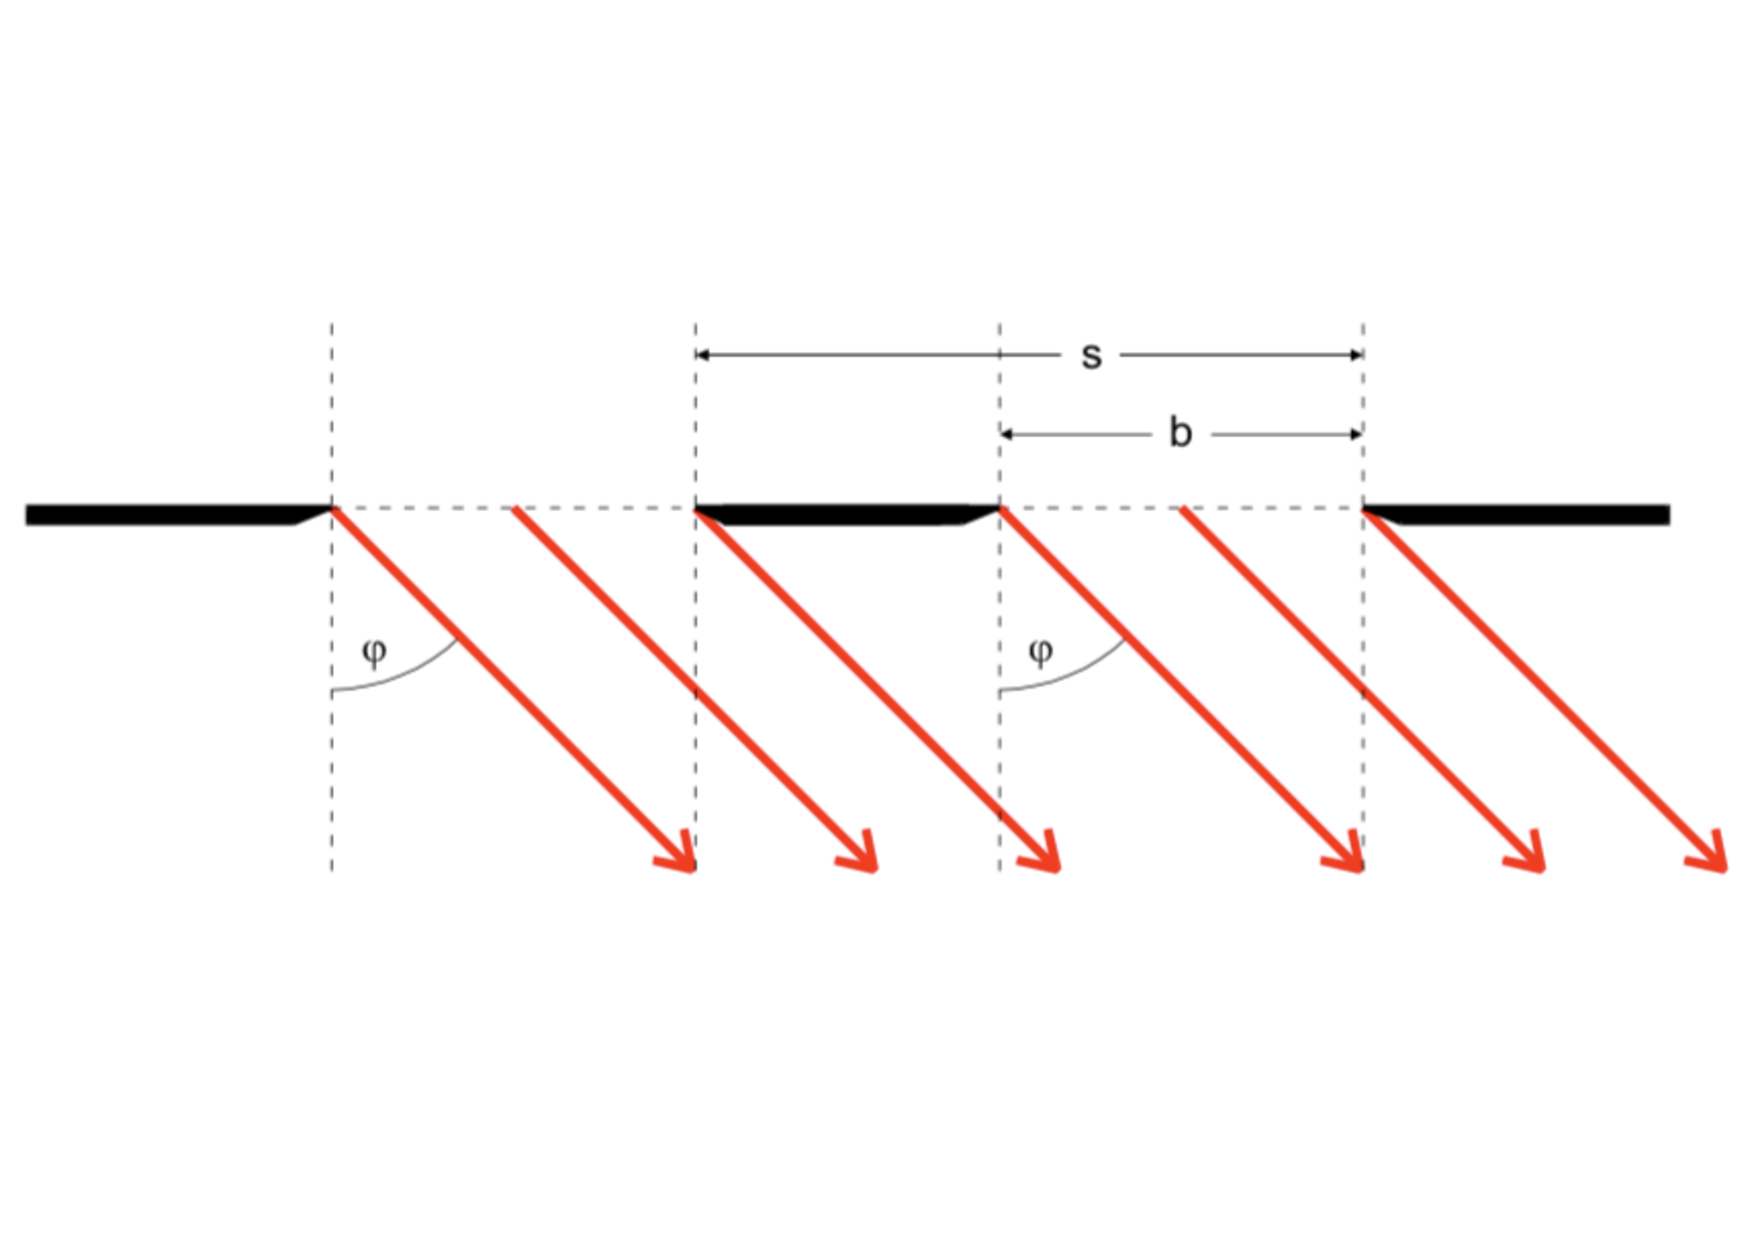
\includegraphics[width=\textwidth]{doppelspalt.pdf}
  \caption{Strahlengang am Doppelspalt \cite{1}}
  \label{fig:doppelspalt}
\end{figure}
Die Intensität eines Spalts des Abstands $b$ verhält sich dann wie folgt:
\begin{align}
  I(\varphi) \propto B^2(\varphi)= 4 \cos^2{ \left( \frac{\pi s \sin{(\varphi)}}{\lambda} \right)} \left( \frac{\lambda}{\pi b \sin{(\varphi)}} \right)^2 \sin^2{\left( \frac{\pi b \sin{(\varphi)}}{\lambda} \right)}.
  \label{eqn:doppelspalt}
\end{align}
Die Intensitätsminima liegen bei
\begin{align*}
  \varphi_{1}(n) &=& \arcsin{\left( \pm \frac{n \lambda}{b} \right)},  &&  n=(1, 2, 3, 4, ...)\\
  \varphi_{2}(k) &=& \arcsin{ \left( \frac{2k+1}{2s} \right)}       ,  &&  k=(0, 1, 2, 3, 4, ...).\\
\end{align*}
%fouriertransformation
\\Mit einer Fouriertransformation lässt sich die Amplitudenverteilung bei der Fraunhofer'schen Beugung allgemeiner beschreiben.
Die Fouriertransformierte hat die Form
\begin{align*}
  g(\zeta)= \int_{-\infty}^{\infty} f(x) \exp{(ix \zeta)} dx = A_{0} \int_{0}^{b} \exp{(ix \zeta)} dx = \frac{A_{0}}{i \zeta}(-1 \exp{(ib\zeta)}).
\end{align*}
Daraus ergibt sich
\begin{align*}
   \zeta = \frac{2 \pi \sin{(\varphi)}}{\lambda}.
\end{align*}
Die Fouriertransformation beschreibt also das Huygens'sche Prinzip mathematisch.

\FloatBarrier
